\documentclass{article}

\usepackage{amsmath}
\usepackage{amsfonts}
\usepackage{graphicx}
\usepackage{float}
\usepackage{hyperref}
\usepackage{subfig}
\usepackage[margin=0.75in]{geometry}

\graphicspath{{./assets/}}

\title{Why are voltage dividers universal to any circuit?}
\author{Igor Krzywda}

\begin{document}

\maketitle

\section{Introduction}

    Voltage divider is an ubiquitous and vesrsitaile electric component. 
    It consists of two resistors connected 
    in series with output terminal between them (See Figure~\ref{fig:divider_0}. 
    If the premise upon which the component works is manipulating two resistances,
    why cannot they be bought as a product? 

    \begin{figure}[H]
        \caption
        \centering
        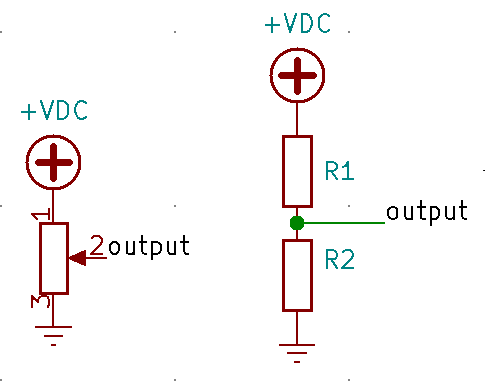
\includegraphics[width=0.1\linewidth]{divider_0}
        \label{fig:divider_0}
    \end{figure}

\section{A voltage divider on its own}
    
    As mentioned in the introduction, a voltage divider are two resistors 
    put in series and the desired output is across one of resistors. A very 
    intuitive example of a voltage divider is a potentiometer, which generally
    is some kind of resistive material with slider on it where the resistance 
    is proportional to the length of the material between slider and terminal
    (See Figure -). Potentiometer will be the basis of subsequent considerations.

\section{Output voltage under no load}

    In order to calculate the output voltage divider will give, we need to 
    use Ohm's law to derive the formula (use figure - as reference). Ohm's 
    law states that $V = IR$, and since our output voltage is found across
    $R_2$, we can find $V_{out}$ by doing the following (Equation~\eqref{eq:vd_no_load})

    \begin{align}
        V_{out} = IR_2, I = \frac{V}{R} \\
        V_{out} = \frac{V_{in}}{R_1 + R_2} \cdot R_2 = V_{in}\frac{R_2}{R_1 + R_2}%
            \label{eq:vd_no_load}
    \end{align}

    From the calculations we could say that the output voltage $V_{out}$ is 
    dependent on the ratio of $R_2$ and the resistance of the whole circuit
    $R_1 + R_2$, and considering the case of potentiometer, where the net
    resistance always amounts to some constant value, the function of $V_{out}$
    with reference to $R_2$ is linear. From this point, it could be wrongly 
    said that in order to step down the voltage to power some component, all
    that needs to be done is to set the dial to desider $R_2$ and plug in 
    the load. This, however is not the case.

\section{Output voltage under load}

    Figure - shows our potentiometer with load connected to the output terminal.
    It is already visible that the load, which has its own resistance is connected
    in parallel to $R_2$ rendering the net resistance of $R_l$ and $R_2$ different, 
    as the resistance calculated for parallel circuit (Equation
    ~\eqref{eq:r_parallel}) will amount to less than the sum of the two 
    resistances. 
    
    \begin{equation}\label{parallel_circuit_R}
        \frac{1}{R} = \frac{1}{R_1} + \frac{1}{R_2} + ... + \frac{1}{R_n} %
            \label{eq:r_parallel}
    \end{equation}
    
    We can derive the formula for this case from equation ~\eqref{eq:vd_no_load} 
    (Equation~\ref{eq:ohm_derived})
    
    \begin{align}
        R_p = (\frac{1}{R_2} + \frac{1}{R_l})^{-1} = \frac{R_2R_l}{R_2 + R_l} \\
        V_{out} = \frac{V_{in} \cdot R_p}{(R_1 + R_p)} \\
        V_{out} = \frac{V_{in}(R_2R_l)}{R_1(R_2 + R_l) + R_2R_l}% 
            \label{eq:ohm_derived}
    \end{align}

    We can see from equation~\eqref{eq:ohm_derived} that the load connected to 
    the potentiometer is an integral part to the circuit that cannot be neglected
    in any way and that it caused the linearity of the voltage output to disappear.

\section{Voltage divider output with different loads}

    Now, let us check the calculations with an experiment. Circuit in figure -
    will be used to generate analog signal by changing the position of the dial
    in a $50k\Omega$ potentiometer with different loads connected to the output
    of the potential divider. The analog signal will be monitored and saved using
    a microcontroller. In order to make a theoretical prediction, a function 
    $V_{out}(R_2)$ will be plotted with the same values using a Python script
    (See Appendix -)

    \subsection{$320\Omega$ load}

        \begin{figure}[H]%
            \centering
            \subfloat[\centering \label{fig:pred_320} prediction]%
                {{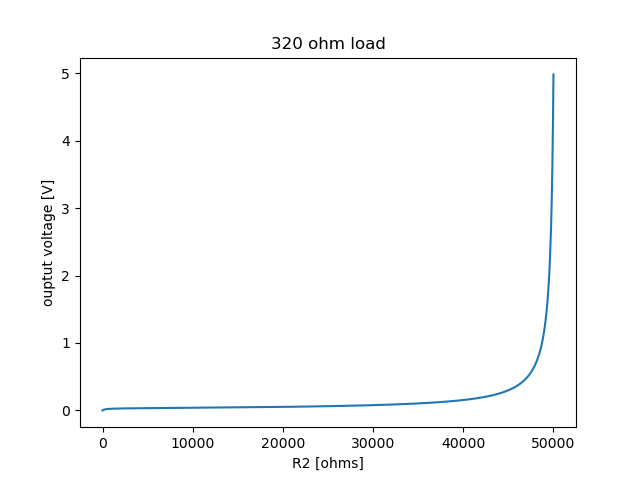
\includegraphics[width=0.4\linewidth]{pred_320.png} }}%
            \qquad
            \subfloat[\centering \label 2]%
                {{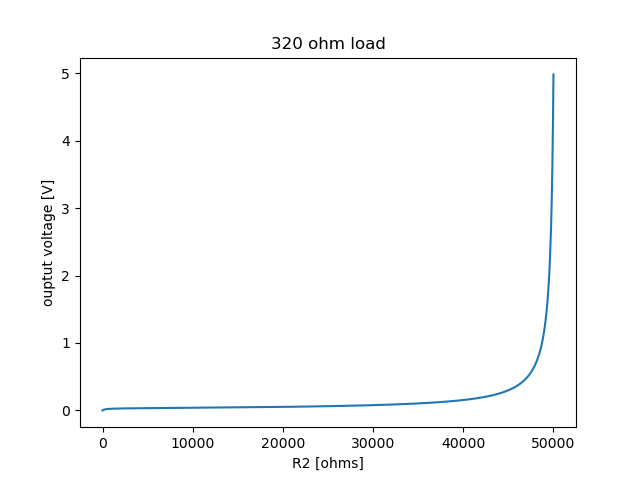
\includegraphics[width=0.4\linewidth]{pred_320.png} }}%
            \label{fig:load_320}%
        \end{figure}


    \subsection{$3220\Omega$ load}

        \begin{figure}[H]%
            \centering
            \subfloat[\centering \label{fig:pred_3220} prediction]%
                {{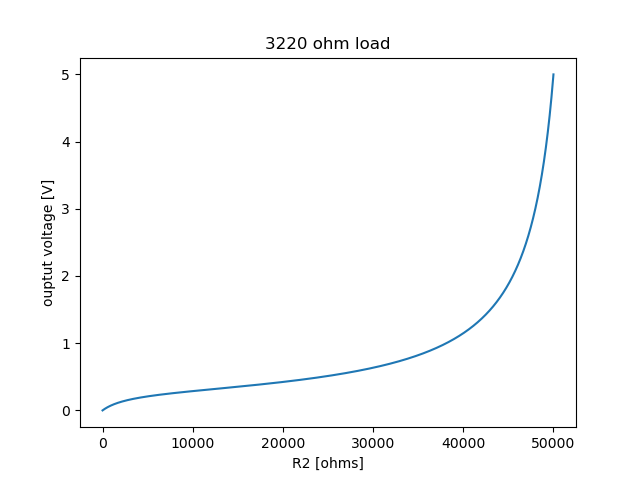
\includegraphics[width=0.4\linewidth]{pred_3220.png} }}%
            \qquad
            \subfloat[\centering \label 2]%
                {{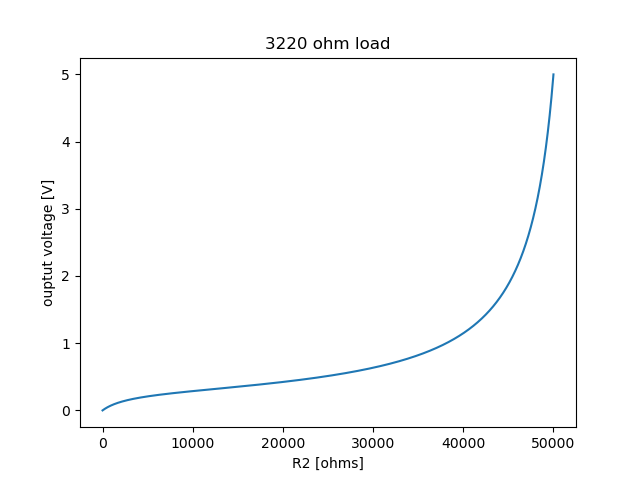
\includegraphics[width=0.4\linewidth]{pred_3220.png} }}%
            \label{fig:load_3220}%
        \end{figure}


    \subsection{$12880\Omega$ load}

        \begin{figure}[H]%
            \centering
            \subfloat[\centering \label{fig:pred_12880} prediction]%
                {{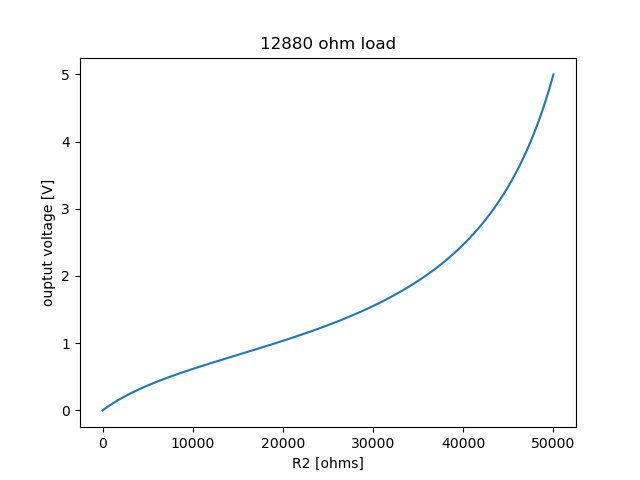
\includegraphics[width=0.4\linewidth]{pred_12880.png} }}%
            \qquad
            \subfloat[\centering \label 2]%
                {{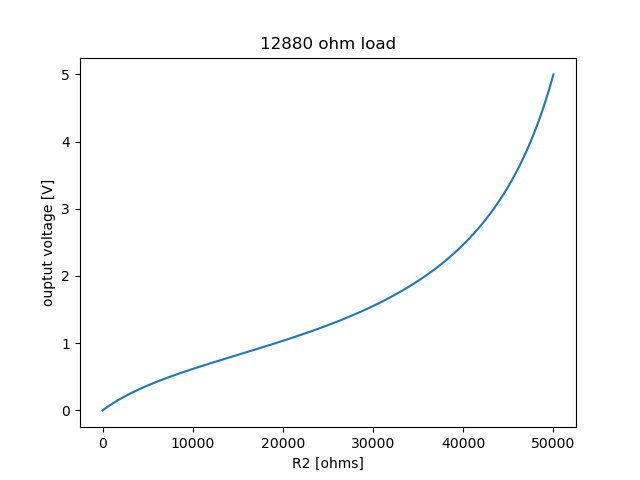
\includegraphics[width=0.4\linewidth]{pred_12880.png} }}%
            \label{fig:load_12880}%
        \end{figure}


    \subsection{$32200\Omega$ load}

        \begin{figure}[H]%
            \centering
            \subfloat[\centering \label{fig:pred_32200} prediction]%
                {{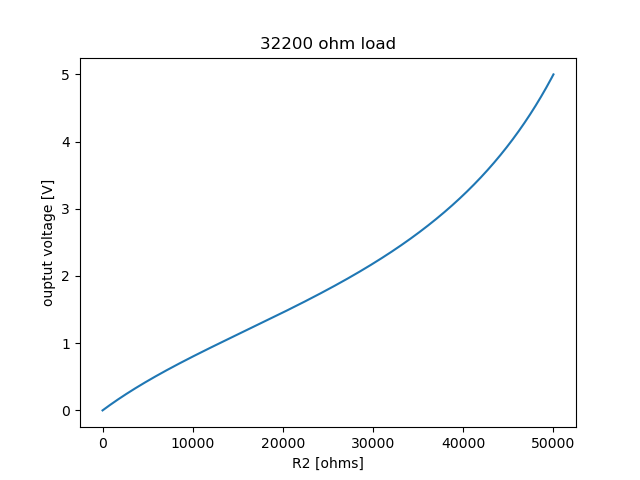
\includegraphics[width=0.4\linewidth]{pred_32200.png} }}%
            \qquad
            \subfloat[\centering \label 2]%
                {{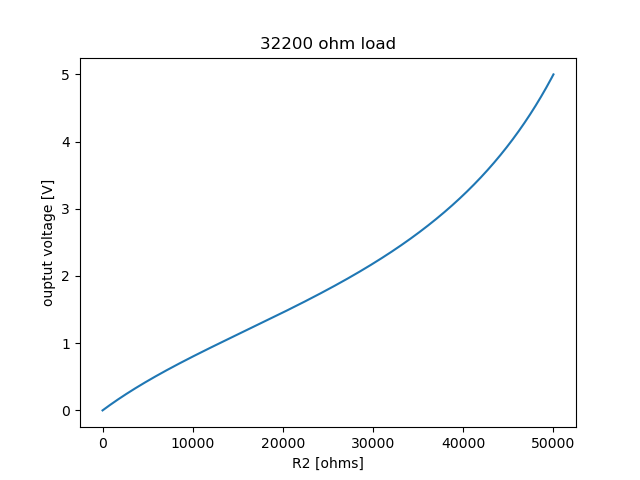
\includegraphics[width=0.4\linewidth]{pred_32200.png} }}%
            \label{fig:load_32200}%
        \end{figure}

\end{document}
